\section{PSF Reconstruction}
	This section contains information about the models and notebooks used to reconstruc PSFs data.

	
	\subsection{Purpose}
	
		The purpose of this project is to check if there are models that can reconstruct PSF data generated from a simulation using PL fluxes.
		
		
	\subsection{Data}
	
		The data related to this project was generated using HCIpy. The main functions used for this are \filename{generate\_psf\_complex\_fields} and \filename{compute\_output\_fluxes\_from\_complex\_field} that can be found in \href{https://github.com/Dacarpe03/PLImageReconstruction/blob/main/Utils/data_utils.py}{data\_utils.py}.\\
		
		These PSFs are generated from atmospheric aberrations, NOT zernike coefficients.\\
		
		There are 90000 datapoints in this project. The paths to them are found in \href{https://github.com/Dacarpe03/PLImageReconstruction/blob/main/Utils/psf_constants.py}{psf\_constants.py}.\\
	
	
	\subsection{Code}

		\begin{itemize}
			\item To generate the data see the notebook \href{https://github.com/Dacarpe03/PLImageReconstruction/blob/main/PSFReconstruction/DataNotebooks/PSFGeneration.ipynb}{PSFGeneration.ipynb}.
			\item To process the data (eg. flatten, compute PSF intensities, crop PSFs) see the notebook \href{https://github.com/Dacarpe03/PLImageReconstruction/blob/main/PSFReconstruction/DataNotebooks/PSFProcessing.ipynb}{PSFProcessing.ipynb}.
			\item To train models check the folder \href{https://github.com/Dacarpe03/PLImageReconstruction/tree/main/PSFReconstruction/Training}{Training}.
			
		\end{itemize}


	\subsection{Results}
		These are some examples of the models, some of them predict amplitude and phase from the PSF, others just its intensity:
		
		\begin{figure*}[ht!]
			\centering
			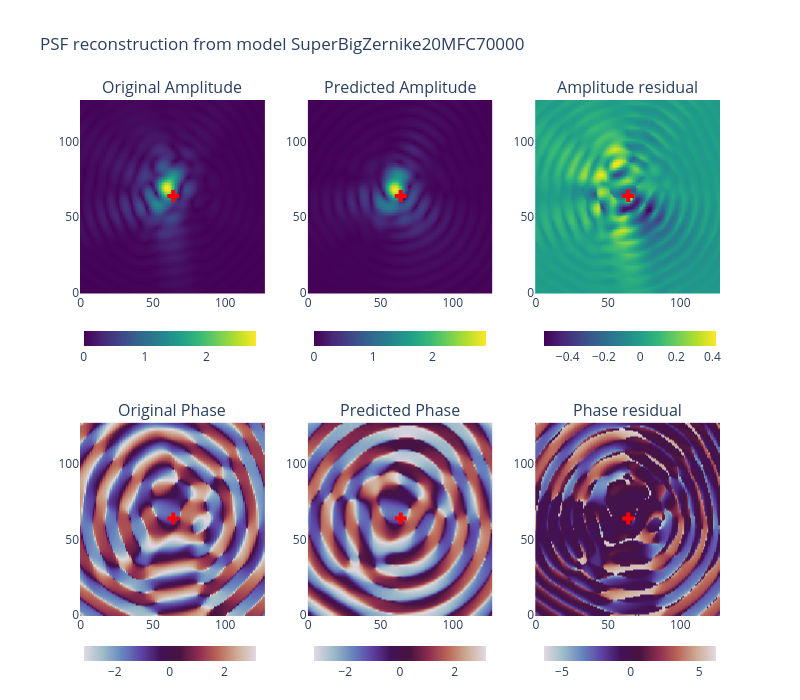
\includegraphics[width=0.9\textwidth]{
		psf-SuperBigZernike20MFC70000-1-validation}
			\caption{Output example from an amplitude+phase predictor}
		\end{figure*}
		
		\begin{figure*}[ht!]
			\centering
			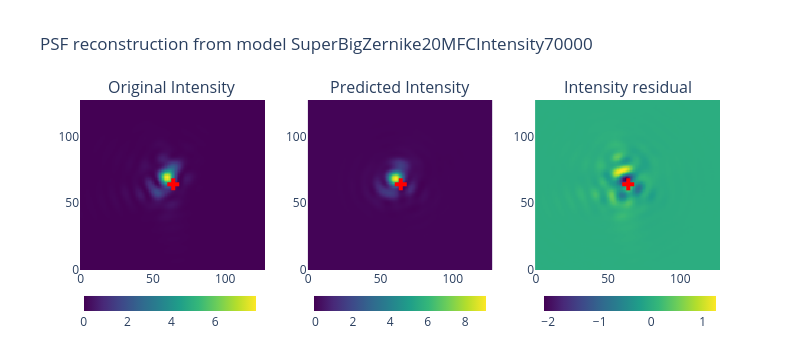
\includegraphics[width=0.9\textwidth]{
		psf-SuperBigZernike20MFCIntensity70000-1-validation}
			\caption{Output example from an intensity predictor}
		\end{figure*}
		\FloatBarrier
		
		To see all architectures, plots and results check PART II from \filename{appendix.pdf}.
	
		